\subsection{实验}
\subsubsection{数据预处理与划分}
实验使用课程任务提供的工业图像异常检测数据，包含榛子（\texttt{hazelnut}）与拉链（\texttt{zipper}）两个产品类别，共602张图像。表\ref{tab:data}展示了数据划分及类别构成。两类各使用200张正常图和50张异常图进行训练，测试集共有72张正常图和30张异常图。

\begin{table}[t]
\caption{课程图像数据划分与类别构成（张）}
\label{tab:data}
\centering
\setlength{\tabcolsep}{4pt}
\begin{tabular}{lrrrrr}
\toprule
&\multicolumn{2}{c}{训练集}&\multicolumn{2}{c}{测试集}&\\
\cmidrule(lr){2-3}\cmidrule(lr){4-5}
产品&正常&异常&正常&异常&合计\\
\midrule
榛子&200&50&40&15&305\\
拉链&200&50&32&15&297\\
合计&400&100&72&30&602\\
\bottomrule
\end{tabular}
\end{table}

程序直接读取课程压缩包，训练标签由\texttt{train/good}和\texttt{train/bad}目录确定，测试真值按产品类别与相对路径关联官方标签文件。核对原始数据可知，602张图像的尺寸均为$1024\times1024$；解码为RGB后的像素哈希均不同，未发现像素完全相同的重复图像。

图\ref{fig:samples}展示的是训练集中的正常与异常图像。榛子异常图003的壳面可见孔洞，拉链异常图006的布边出现缺损。这些差异可能仅占图像的一小部分，因此采用整图表示与局部表示共同评分。图\ref{fig:features}展示同一榛子图像的多层特征响应。随网络层次加深，空间网格逐步变粗，不同层提供不同尺度的外观线索。

\begin{figure*}[t]
\centering
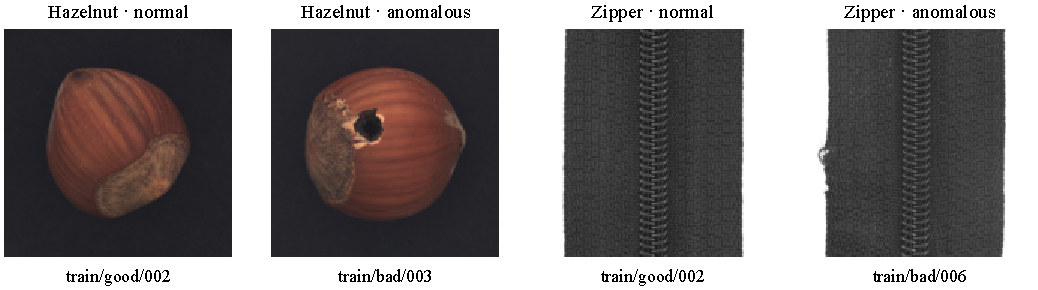
\includegraphics[width=\textwidth]{figures/training-samples.pdf}
\caption{课程训练集的正常与异常样例。编号对应产品类别及训练标签目录内的文件名。}
\Description{榛子正常002、异常003以及拉链正常002、异常006四张训练图像。}
\label{fig:samples}
\end{figure*}

\begin{figure*}[t]
\centering
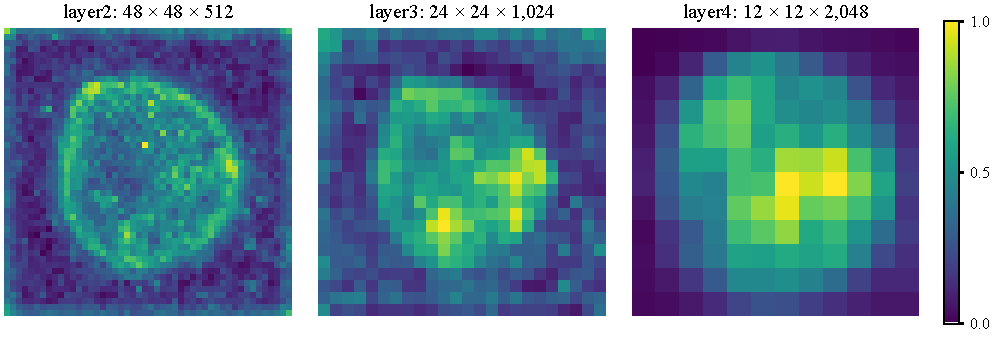
\includegraphics[width=\textwidth]{figures/feature-responses.pdf}
\caption{正常榛子训练图002的多层特征响应。各层按通道求均值并独立作最小值—最大值归一化，颜色强度仅在同一子图内比较。}
\Description{layer2、layer3、layer4的特征响应示例。}
\label{fig:features}
\end{figure*}

\subsubsection{实验配置与拟合流程}
每类训练集进行五折划分，每折使用160张正常图和40张异常图拟合，对另40张正常图与10张异常图计算折外分数。表\ref{tab:config}给出候选参数与最终配置。每类依次评估4组SVM参数、3个局部聚合比例和5个融合权重，共12组候选；两类合计24组。该过程为分阶段选择，并非所有参数的笛卡尔积联合搜索。

\begin{table*}[t]
\caption{检测分支、特征表示与融合配置}
\label{tab:config}
\centering
\begin{tabular}{lll}
\toprule
模块&设置或候选范围&两类最终配置\\
\midrule
共享特征&Wide ResNet50-2，ImageNet-1K V1&冻结参数；输入$384\times384$\\
全局特征&三层均值池化与最大池化&7168维；逐维标准化\\
局部特征&两层拼接与固定高斯投影&$2304\times256$；投影种子2026\\
SVM&$C\in\{1,10\}$，$\gamma\in\{0.1,1\}/7168$&$C=10$，$\gamma=0.1/7168$\\
正常记忆库&正常局部描述子随机无放回采样&8192个描述子；8 MiB\\
局部聚合&$q\in\{0.005,0.01,0.02\}$&$q=0.01$；最高24个距离取均值\\
分数融合&$\alpha\in\{0,0.125,0.25,0.5,1\}$&全局权重0.875；局部权重0.125\\
交叉验证&分层五折；划分种子42&每类250个折外分数\\
融合阈值&在训练集折外分数上确定&榛子\HazThreshold；拉链\ZipThreshold\\
\bottomrule
\end{tabular}
\end{table*}

实验在Windows 11、Python \RunPython、CPU环境下重新执行，使用PyTorch \RunTorch、Torchvision \RunVision{}及scikit-learn \RunSklearn，设置\RunThreads 个计算线程、每批\RunBatch 张图像。从原始图像提取特征、进行五折选参、全量重拟合及测试评价共耗时\RunMinutes 分钟。下文表格由本次运行保存的预测和指标文件生成，图表使用同一份完整精度结果。

\subsubsection{评价指标}
评价将异常图像作为正类。记真正例、真负例、假正例和假负例数分别为TP、TN、FP和FN，总样本数为$N$。固定阈值下的指标定义为
\begin{equation}
\begin{aligned}
 \mathrm{Accuracy}&=\frac{\mathrm{TP}+\mathrm{TN}}{N},\\
 \mathrm{Precision}&=\frac{\mathrm{TP}}{\mathrm{TP}+\mathrm{FP}},\quad
 \mathrm{Recall}=\frac{\mathrm{TP}}{\mathrm{TP}+\mathrm{FN}},\\
 F1&=\frac{2\mathrm{TP}}{2\mathrm{TP}+\mathrm{FP}+\mathrm{FN}}.
\end{aligned}
\label{eq:metrics}
\end{equation}
准确率描述全部图像的正确比例，精确率描述异常预测中的真实异常比例，召回率描述异常图像的检出比例。F1综合精确率与召回率，没有预测异常时将精确率与F1记为0。

平衡准确率对两类正确识别率赋予相同权重：
\begin{equation}
 \mathrm{BA}=\frac12\left(\frac{\mathrm{TP}}{\mathrm{TP}+\mathrm{FN}}
 +\frac{\mathrm{TN}}{\mathrm{TN}+\mathrm{FP}}\right).
 \label{eq:ba}
\end{equation}
连续分数使用AUROC和平均精确率（AP）评价排序质量；在类别比例不均衡时，PR曲线有助于观察异常预测的精确率与召回率\cite{saito}。设正类、负类索引集合分别为$\mathcal P$和$\mathcal N$，对应样本数为$n_+$与$n_-$，则
\begin{equation}
\begin{aligned}
\mathrm{AUROC}=\frac1{n_+n_-}\sum_{i\in\mathcal P}\sum_{j\in\mathcal N}
\bigl[&\ind(S_i>S_j)\\[-2pt]
&+\tfrac12\ind(S_i=S_j)\bigr].
\end{aligned}
\label{eq:auroc}
\end{equation}
同分样本对按半次正确排序计。AP按召回率增量对精确率加权：
\begin{equation}
 \mathrm{AP}=\sum_\ell(R_\ell-R_{\ell-1})P_\ell,\quad R_0=0.
 \label{eq:ap}
\end{equation}
其中$P_\ell,R_\ell$对应阈值逐渐降低时的工作点，同分图像同时纳入。AP采用阶梯加权，不使用梯形面积近似。由于两个产品独立建模，AUROC与AP按产品报告；总体分类指标由各产品采用自身阈值后的混淆计数汇总计算。

\subsubsection{总体效果与独立分支对照}
表\ref{tab:results}展示恒判正常、全局SVM、局部最近邻和融合方法的测试集结果。各检测分支采用训练阶段确定的阈值。融合方法正确判断榛子55/55张、拉链47/47张，合计102/102张，72张正常图与30张异常图均正确分类。

\begin{table*}[t]
\caption{独立检测分支与融合方法的课程固定测试集结果}
\label{tab:results}
\centering
\setlength{\tabcolsep}{5pt}
% Generated from test_metrics.csv; do not edit the numerical rows manually.
\begin{tabular}{llrrrrrrr}
\toprule
产品&方法&正确数&Accuracy (\%)&Precision&Recall&F1&AUROC&AP\\
\midrule
榛子&恒判正常&40/55&72.73&0.0000&0.0000&0.0000&0.5000&0.2727\\
&全局SVM&54/55&98.18&0.9375&1.0000&0.9677&1.0000&1.0000\\
&局部最近邻&55/55&100.00&1.0000&1.0000&1.0000&1.0000&1.0000\\
&融合&55/55&\textbf{100.00}&\textbf{1.0000}&\textbf{1.0000}&\textbf{1.0000}&\textbf{1.0000}&\textbf{1.0000}\\
\midrule
拉链&恒判正常&32/47&68.09&0.0000&0.0000&0.0000&0.5000&0.3191\\
&全局SVM&46/47&97.87&0.9375&1.0000&0.9677&1.0000&1.0000\\
&局部最近邻&45/47&95.74&0.8824&1.0000&0.9375&0.9875&0.9749\\
&融合&47/47&\textbf{100.00}&\textbf{1.0000}&\textbf{1.0000}&\textbf{1.0000}&\textbf{1.0000}&\textbf{1.0000}\\
\bottomrule
\end{tabular}

\par\smallskip
{\footnotesize 粗体标出融合方法。各方法使用自身训练内阈值，未用测试标签重新选阈值。}
\end{table*}

全局SVM与局部最近邻均正确判断100/102张，总体准确率为98.04\%；融合后提高至100\%，增加1.96个百分点。榛子融合结果与局部分支持平；拉链融合相较全局和局部分支分别多正确判断1张和2张，F1分别提高0.0323和0.0625。

\begin{figure*}[t]
\centering
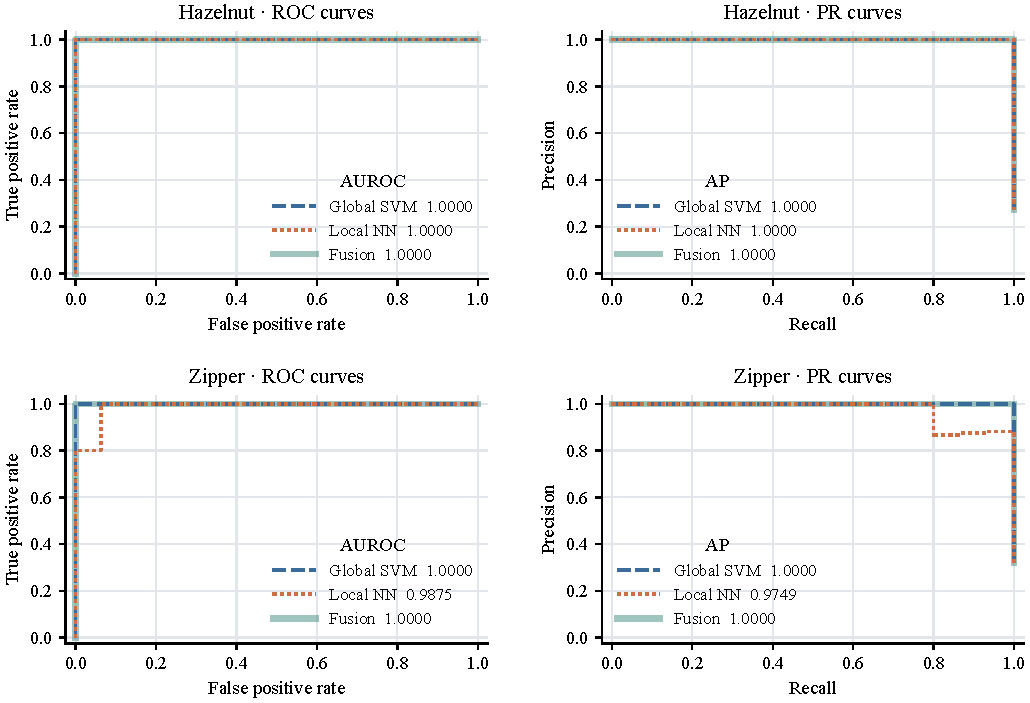
\includegraphics[width=\textwidth]{figures/roc-pr-curves.pdf}
\caption{两类产品的ROC和PR曲线。Global SVM、Local NN和Fusion分别表示全局、局部和融合方法；排序相同时曲线重合。}
\Description{榛子和拉链的ROC与PR曲线，展示全局、局部与融合分支的排序质量。}
\label{fig:curves}
\end{figure*}

恒判正常基线的总体准确率仍达到$72/102=70.59\%$，但漏掉全部30张异常，召回率和F1均为0，BA为0.5。因此，准确率应与异常召回率、误报数及漏检数共同解读。

\subsubsection{误报、漏检与分支互补}
图\ref{fig:confusion}展示各方法的总体混淆矩阵。全局与局部分支均有70个TN、2个FP、0个FN和30个TP，精确率为$30/32=0.9375$，召回率为1，F1为0.9677，BA为0.9861。融合后TN增加至72，FP降为0；异常检出数保持30。

\begin{figure*}[t]
\centering
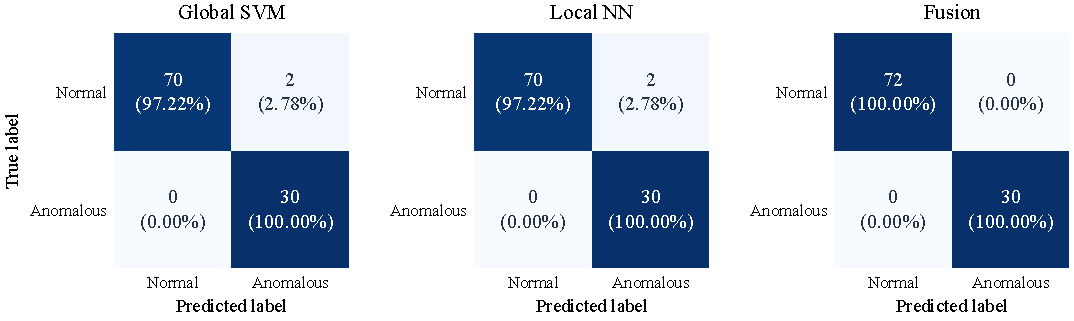
\includegraphics[width=\textwidth]{figures/confusion-matrices.pdf}
\caption{三个检测方法的总体混淆矩阵。Normal为正常、Anomalous为异常；行表示真实类别，列表示预测类别，括号内为该类别的比例。}
\Description{全局与局部分支均有两次误报，融合无误报与漏检。}
\label{fig:confusion}
\end{figure*}

两个独立分支虽然总体正确数相同，误报对象却不同。全局分支误报正常榛子032和正常拉链029；局部分支误报正常拉链023和036。图\ref{fig:errors}给出这四张图的判定对照，两支错误对象没有重叠，融合后全部恢复为正常。

\begin{figure}[t]
\centering
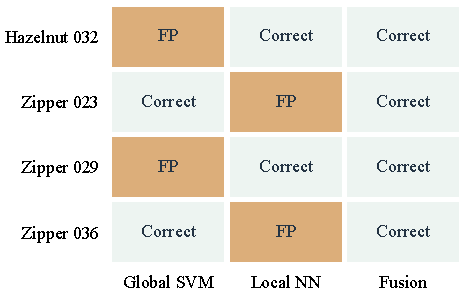
\includegraphics[width=\columnwidth]{figures/error-complementarity.pdf}
\caption{四张正常图像在各分支下的误报情况。FP表示误报，Correct表示正确判为正常。}
\Description{全局误报榛子032和拉链029，局部误报拉链023和036，融合均正确。}
\label{fig:errors}
\end{figure}

全局分支汇总整图外观，局部分支比较单个位置与正常记忆库的差异，因此同一张图可能在两种表示下得到不同响应。该对照说明两支在本测试集上的错误具有互补性。融合使用训练内确定的尺度、权重和阈值共同决定最终标签，其收益体现在减少正常图误报。

\subsubsection{排序质量与阈值余量}
图\ref{fig:curves}展示各方法的ROC与PR曲线。榛子三个分支的曲线重合，拉链局部分支的AUROC为\ZipLocalAUC、AP为\ZipLocalAP，说明存在少量正常与异常样本的排序交错。两类全局分支的AUROC和AP均为1，但固定阈值下仍各误报一张正常图。排序指标衡量异常分数相对于正常分数的位置，分类结果还取决于阈值落在何处。

对每个产品，取融合分数最高的正常图与最低的异常图。表\ref{tab:boundary}给出四个边界样本，定义阈值余量为$\Delta=S_c-\tau_c$。负值对应正常判定，非负值对应异常判定。

\begin{table*}[t]
\caption{各产品中最接近分类间隙的正常与异常样本}
\label{tab:boundary}
\centering
% Generated from full-precision scores; round only for display.
\begin{tabular}{llrrr}
\toprule
产品及测试编号&真实类别&融合分数$S_c$&阈值$\tau_c$&余量$\Delta$\\
\midrule
榛子032&正常&1.359186&1.507247&$-0.148061$\\
榛子004&异常&1.693860&1.507247&$+0.186613$\\
拉链029&正常&0.933833&0.950929&$-0.017097$\\
拉链007&异常&1.520392&0.950929&$+0.569463$\\
\bottomrule
\end{tabular}

\par\smallskip
{\footnotesize 三个数值字段由本次完整精度结果分别保留六位小数；展示值相减可能存在末位舍入差。}
\end{table*}

图\ref{fig:scores}展示两类产品的融合分数分布。正常样本集中在各自阈值左侧，异常样本位于右侧，横轴上的短线给出逐图分数位置。拉链\ZipNormalID 的余量绝对值仅\ZipNormalMarginAbs，接近该产品的判定边界。其全局分数为$\ZipNormalGlobalScore$，高于全局阈值$\ZipNormalGlobalThreshold$，因此被全局分支误报；局部分数为\ZipNormalLocalScore，低于局部阈值\ZipNormalLocalThreshold。两支校准融合后，该图回到正常一侧。

\begin{figure*}[t]
\centering
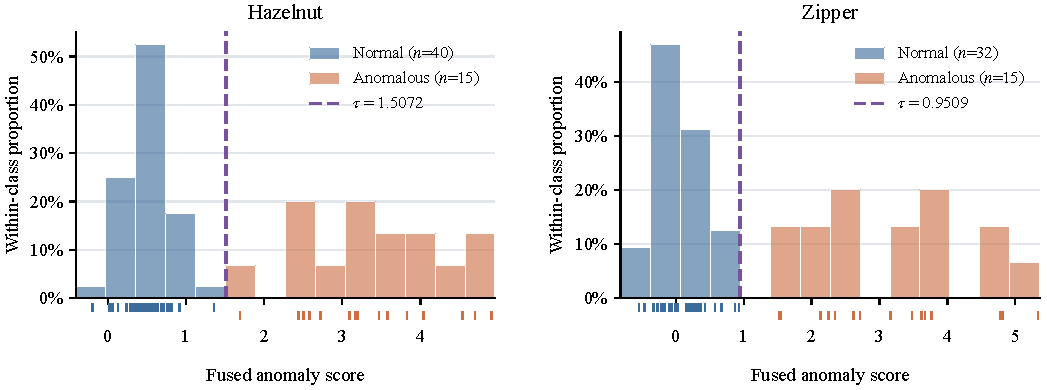
\includegraphics[width=\textwidth]{figures/score-distribution.pdf}
\caption{正常与异常图像的融合分数分布。Normal为正常、Anomalous为异常；纵轴按真实类别归一化，短线表示单张图像，虚线为训练内阈值。}
\Description{榛子和拉链的实际融合分数分布，各产品分别使用自身评分尺度与阈值。}
\label{fig:scores}
\end{figure*}

榛子的最高正常分数和最低异常分数分别位于阈值两侧，余量绝对值为\HazNormalMarginAbs 和\HazAbnormalMarginAbs；拉链最低异常分数高于阈值\ZipAbnormalMarginAbs。余量可用于识别需要优先复查的样本，但并非校准概率，不宜直接跨产品比较。

\subsubsection{边界样本与局部热图}
图\ref{fig:heatmap}展示四个边界样本的原图与局部最近邻热图。使用本次冻结模型重新计算各位置相对于正常记忆库的距离，并按单张图距离场的第99百分位数归一化后截断至$[0,1]$。该显示尺度表示图内的相对响应，不同图之间的颜色强弱不能直接比较。

\begin{figure*}[t]
\centering
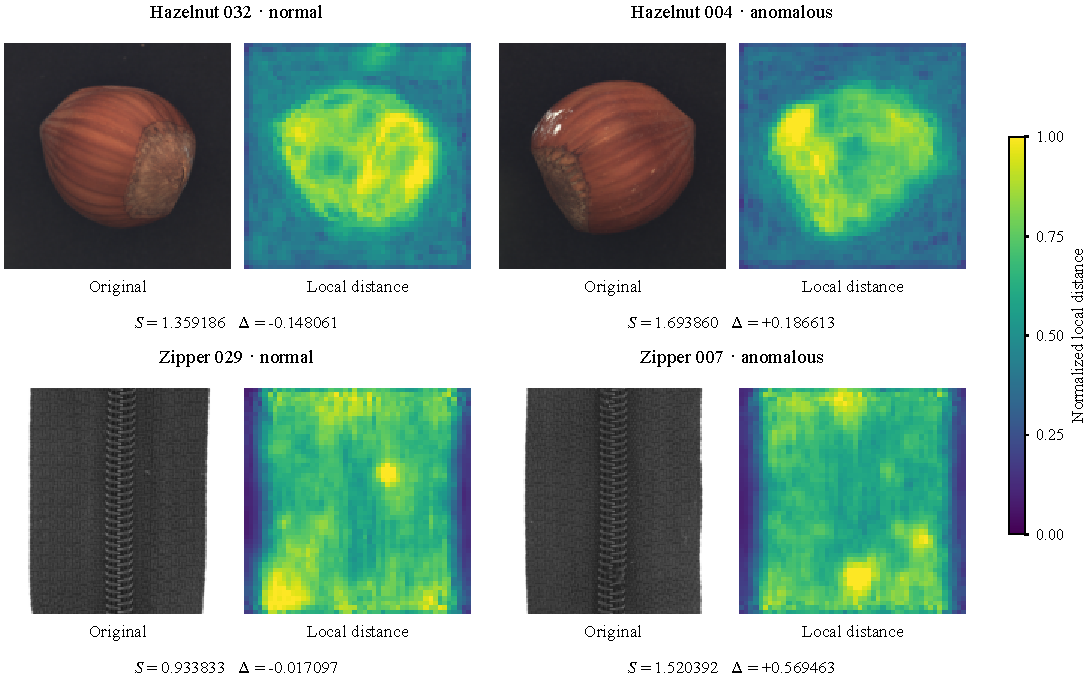
\includegraphics[width=\textwidth]{figures/qualitative-heatmaps.pdf}
\caption{边界样本的原图与局部异常响应。每组左侧为原图，右侧为热图；图像级标签由融合分数和固定阈值共同决定。}
\Description{榛子032、榛子004、拉链029和拉链007的原图与热图成对展示。}
\label{fig:heatmap}
\end{figure*}

异常榛子004在左上方浅色痕迹附近具有较强响应，正常榛子032在果壳与底部纹理交界处也出现响应。局部距离既可能响应缺陷，也可能响应记忆库中覆盖不足的自然纹理，因此高响应区域本身不等同于异常标签。融合后，正常032位于阈值的正常一侧，异常004位于异常一侧。

正常拉链029的局部分数低于局部阈值，与全局分支形成分歧，融合后被判为正常。异常拉链007在下部齿列与部分边缘处出现响应，其融合分数\ZipAbnormalScore 高于阈值\ZipThreshold，最终判为异常。课程数据提供的是图像级真值，本实验据此评价图像检测效果，热图仅用于定性回查，不报告像素级定位指标。

\subsubsection{结果核验与适用范围}
为核对训练、预测与报告之间的一致性，使用保存的模型从102张原始测试图像重新提取特征，复算三个分支共306个分数，最大绝对差为0。根据留存的折外分数复算24组参数候选、阈值和分位数校准统计量，所得选择与冻结配置一致。评价指标另由混淆计数、正负样本两两排序和同分组累计独立计算，8组结果全部一致。

本实验的100\%准确率对应课程给定的102张测试图像。该测试集在项目早期曾用于比较版本，因而当前代码在测试前冻结配置，并不意味着整个开发过程从未接触测试结果。每类测试集仅含15张异常，增加一次漏检就会使该类召回率下降约6.67个百分点。新产品批次、拍摄条件变化及未见缺陷仍需要独立测试。

训练与核验保存逐图分数、评价指标、折外参数选择记录及冻结配置。代码结构、环境配置和执行命令见随附源码说明。
